\begin{figure*}[t]
\centering
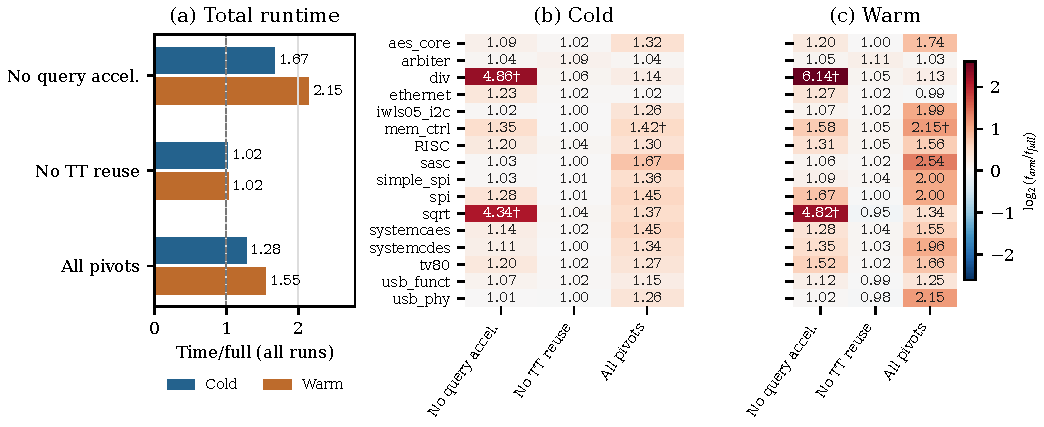
\includegraphics[width=\textwidth]{results/build_ablation.pdf}
\caption{Query, truth-table and pivot-control runtime relative to full, cold/warm: aggregate optimizer-time ratios and per-design ratios. Colors encode the logarithm of each ratio. $\dagger$ marks at least one TO; equal elapsed budgets do not imply equal completed work. Selected-output area effects and timeout counts appear in \Cref{tab:ablation}.}\label{fig:ablation}
\end{figure*}

\begin{figure}[t]
\centering
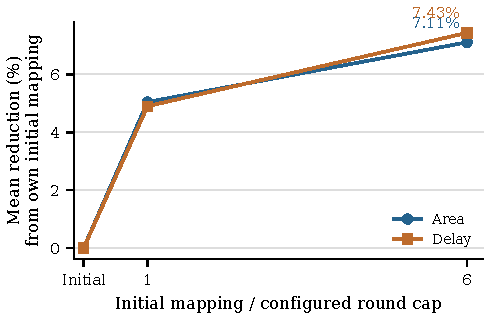
\includegraphics[width=.90\linewidth]{results/round_progress.pdf}
\caption{Selected-output reductions from $N_e$ at caps 1 and 6. Cold/warm curves separate when different; intermediate caps were not measured.}\label{fig:rounds}
\end{figure}
\section{Experimental Results}

\MfsComparisonTable
\MainResultTable
\subsection{Setup}\label{sec:setup}
We evaluate sixteen designs with the ASAP7 genlib~\cite{asap7}, reporting area in $\mu m^2$ and worst-output delay in ps. We use C++/mockturtle~\cite{EPFLLibraries}, Rust/\textit{egg}~\cite{willsey2021egg}, and ABC~\cite{ABCTool}.

All experiments fix the initial delay bound across rounds (\Cref{eq:objective}), with whole-window synthesis and unmap/remap exploration disabled.

For \texttt{mfs3}, both tools use the same 40-entry subset with at most six inputs per cell, and byte-identical area-oriented \texttt{emap} inputs. The evaluated \texttt{mfs3} implementation restricts cell truth tables and node simulation to six inputs. Preprocessing experiments and ablations use all 47 entries for initial mapping and optimization.

The direct input $N_i$ maps the raw AIG without ABC optimization. For $N_e$, the flow repeats \texttt{fraig; resyn2rs; fraig; compress2rs} until the AND count stops decreasing, with a 20-iteration cap, then applies area-oriented \texttt{emap}. Let $A_e=A(N_e)$ and $D_e=D(N_e)$.

Cuts use $K=6$, $B=12$ and $\theta=0$. Care uses an eight-input reconvergence window and 60\,s cumulative budget, then full care; SAT refinement is off. The three-level database has area cap $0.50$. SOP/DSD starts at four leaves; Shannon/Davio at three, with two ranked pivots per family. Each native structure cache holds 262144 entries. Independent polarity factoring and exact AIG synthesis are off. L4 allows two iterations, 500 e-nodes, eight realizations per class, 20000 combinations and 4000 visits. Chain blocks have two steps and minimum length six. Round caps allow early stopping.

Experiments run on two Xeon Gold 6226R sockets (32 cores), Ubuntu 22.04.5, GCC 11.2.0, Rust 1.99.0 and ABC 1.01. A shared host runs up to twelve single-worker ePMapping optimizations and six independent ABC jobs. Both tools have a 1000\,s post-mapping limit. For ePMapping this includes optimizer preparation, all rounds and final rebuild, excluding preprocessing, mapping and CEC. An outer 3600\,s guard covers setup and validation.

Each configuration/design runs cold with an empty private pool, then warm with the same pool and limits. Native caches restart; OS caches are not cleared. Both groups share the verified ABC batch. Times are $t_c/t_w$. Externally interrupted attempts are archived, excluded from timing totals, and retried with their prescribed cache state.

Completed and selected deadline outputs undergo CEC and independent serialized-PPA audits. A TO remains incomplete: the best legal checkpoint is selected, or the initial mapping. Snapshot costs count toward 1000\,s; post-run validation does not. Interrupted ABC runs retain the initial mapping. \FullCompletionSentence{} Across all parts, cold/warm have \ColdCompleted{}/\WarmCompleted{} completions and \ColdMethodTimeouts{}/\WarmMethodTimeouts{} timeouts; \ColdCheckpointSelections{}/\WarmCheckpointSelections{} timeouts select improved checkpoints. Differing costs are stacked or separated by a slash, cold first. Define $\delta A_j=100(A_j/A_{0,j}-1)$ and $\delta D_j=100(D_j/D_{0,j}-1)$. Means include initial selections; ablations sum $\Delta A=\sum_j(A_{\rm arm,j}-A_{\rm full,j})$.

\subsection{Area Recovery after AIG Preprocessing}\label{sec:aspdac}

Both preprocessing-experiment caps start from $N_e$ (\Cref{tab:main}). At one round, mean area changes are \OwnOneArea\%; mean delay changes are \OwnOneDelay\% (cold/warm). At cap 6, these are \OwnArea\% area and \OwnDelay\% delay, with \ColdMainCompleted{}/\WarmMainCompleted{} completed runs. Area decreases on \OwnAreaWins{} of sixteen; all selected outputs meet the initial bounds. The caps are measured independently.

For \texttt{arbiter}, area changes from $557.72$ to $\ArbiterArea\,\mu m^2$ and delay from $999.87$ to $\ArbiterDelay$\,ps. The other fifteen average \mbox{\OwnOtherArea\%} area and \mbox{\OwnOtherDelay\%} delay changes.



ASPDAC'25 costs are reconstructed from its reported starts and rounded changes~\cite{aspdac25}; its implementation is unavailable. Our final area is smaller on \MainWins{} designs, with mean area and delay differences of \mbox{\MainAreaAll\%} and \mbox{\MainDelayAll\%}. These approximate comparisons use different starts and cannot isolate post-mapping gains; our delay bound refers to our input.

\subsection{Common-Input Comparison with ABC}\label{sec:mfs3}
Both tools receive the same direct mapping (\Cref{tab:mfs3}); ours uses one round. ABC's \texttt{mfs3 -a} does not enforce our initial-delay bound, so we distinguish raw and externally guarded outputs.

ABC completes \ABCCompleted{} designs and times out on \ABCTimeouts{}. On the ABC-completed subset, its mean area/delay changes are \mbox{\ABCArea\%}/\mbox{\ABCDelay\%}, versus \mbox{\PairedOwnArea\%}/\mbox{\PairedOwnDelay\%} for our verified selections. ePMapping completes \ColdMfsCompleted{}/\WarmMfsCompleted{} designs cold/warm. Its all-sixteen selected-output means are \mbox{\MfsOwnArea\%}/\mbox{\MfsOwnDelay\%}, within the initial delay bounds.

Of the completed ABC outputs, \ABCViolations{} violate the delay bound and \ABCFeasible{} satisfy both bounds. An external guard retains only feasible outputs, otherwise selecting the initial mapping; its paired means are \mbox{\ABCGuardArea\%} area and \mbox{\ABCGuardDelay\%} delay. This guard leaves ABC unchanged.

Ratios in \Cref{tab:mfs3} use each tool's native initial costs: ABC import may normalize output buffers. Times exclude CEC; ABC includes import and writing, ours optimizer preparation through rebuild.

\subsection{Operator Ablations and Efficiency}\label{sec:oracles}
\AblationResultTable


All nineteen arms use identical $N_e$ starts and bounds (\Cref{tab:ablation}); L1 stays enabled. noSYN removes L3, noEGG removes L4, noDB removes lookup and database-derived mapper entries, and noCARE supplies full care. noCHAIN skips composition; noSHARE clears chain memo tables between roots. noNARROW removes narrow initialization; noPHASE disables physical phase reuse.

noSHANNON retains Davio only; noDAVIO retains Shannon only. noREUSE removes forward INV lookup but keeps backward cancellation; noPRICE removes contextual pricing while preserving physical reuse. noQUERY restores uncached inverse queries and dependency traversal. noTRUTH disables decoded simulation and dynamic-table reuse; the common scalar cut memo remains. allPIVOTS removes the pivot cap. cache64K uses 65536 native entries, noAIGREUSE disables pre-mapping AIG reuse, and noLIBSHARE copies libraries.

The noQUERY and noTRUTH time/full ratios are \QueryColdRatio{}/\QueryWarmRatio{} and \TruthColdRatio{}/\TruthWarmRatio{}. allPIVOTS has ratio \PivotColdRatio{}/\PivotWarmRatio{} and summed area differences \PivotAreaCold{}/\PivotAreaWarm{}\,$\mu m^2$. noTRUTH leaves every final area and delay unchanged. Unrestricted pivots recover more area overall but time out on \texttt{mem\_ctrl} cold and warm (\Cref{fig:ablation}).

Removing Shannon and Davio gives summed area differences of \DeltaShannon{} and \DeltaDavio\,$\mu m^2$; removing forward reuse and live pricing gives \DeltaReuse{} and \DeltaPrice\,$\mu m^2$. \UsbAblationExample{} Independent runs can follow different trajectories under care budgets and deadlines. \DeadlineExample{}

noDB improves \DBBetterCount{} designs but changes both lookup and inner mapping. Ablation effects are not additive.

Removing L4 worsens area on \EggWorseCount{} designs; its cold/warm time ratios are \ColdNoEggRatio{}/\WarmNoEggRatio{}. L4 takes \TimeEggShare\%/\WarmTimeEggShare\% of recorded phase time in \ColdPhaseRuns{}/\WarmPhaseRuns{} completed full runs (CEC and other phases excluded). Pool hits avoid saturation and extraction; native caches restart per process. TO ratios compare elapsed budgets, not equal completed work. \CacheDeadlineExample{} Shared-host scheduling affects elapsed time.

